\documentclass[11pt]{article}

%%%%%%%%%%%%%%%%%%%%%%%%%%%%%%%%%%%%%%%%%%%%%%%%%%%%%%%%%%%%%%%%%%%%%%%%%%%%%%%%
% LaTeX Imports
%%%%%%%%%%%%%%%%%%%%%%%%%%%%%%%%%%%%%%%%%%%%%%%%%%%%%%%%%%%%%%%%%%%%%%%%%%%%%%%%
\usepackage{amsfonts}                                                   % Math fonts
\usepackage{amsmath}                                                    % Math formatting
\usepackage{amssymb}                                                    % Math formatting
\usepackage{amsthm}                                                     % Math Theorems
\usepackage{arydshln}                                                   % Dashed hlines
\usepackage{attachfile}                                                 % AttachFiles
\usepackage{cancel}                                                     % Cancelled math
\usepackage{caption}                                                    % Figure captioning
\usepackage{color}                                                      % Nice Colors
\input{./lib/dragon.inp}                                                % Tikz dragon curve
\usepackage[ampersand]{easylist}                                        % Easy lists
\usepackage{fancyhdr}                                                   % Fancy Header
\usepackage[T1]{fontenc}                                                % Specific font-encoding
%\usepackage[margin=1in, marginparwidth=2cm, marginparsep=2cm]{geometry} % Margins
\usepackage{graphicx}                                                   % Include images
\usepackage{hyperref}                                                   % Referencing
\usepackage[none]{hyphenat}                                             % Don't allow hyphenation
\usepackage{lipsum}                                                     % Lorem Ipsum Dummy Text
\usepackage{listings}                                                   % Code display
\usepackage{marginnote}                                                 % Notes in the margin
\usepackage{microtype}                                                  % Niceness
\usepackage{lib/minted}                                                 % Code display
\usepackage{multirow}                                                   % Multirow tables
\usepackage{pdfpages}                                                   % Include pdfs
\usepackage{pgfplots}                                                   % Create Pictures
\usepackage{rotating}                                                   % Figure rotation
\usepackage{setspace}                                                   % Allow double spacing
\usepackage{subcaption}                                                 % Figure captioning
\usepackage{tikz}                                                       % Create Pictures
\usepackage{tocloft}                                                    % List of Equations
%%%%%%%%%%%%%%%%%%%%%%%%%%%%%%%%%%%%%%%%%%%%%%%%%%%%%%%%%%%%%%%%%%%%%%%%%%%%%%%%
% Package Setup
%%%%%%%%%%%%%%%%%%%%%%%%%%%%%%%%%%%%%%%%%%%%%%%%%%%%%%%%%%%%%%%%%%%%%%%%%%%%%%%%
\hypersetup{%                                                           % Setup linking
    colorlinks=true,
    linkcolor=black,
    citecolor=black,
    filecolor=black,
    urlcolor=black,
}
\RequirePackage[l2tabu, orthodox]{nag}                                  % Nag about bad syntax
\renewcommand*\thesection{\arabic{section} }                             % Reset numbering
\renewcommand{\theFancyVerbLine}{ {\arabic{FancyVerbLine} } }              % Needed for code display
\renewcommand{\footrulewidth}{0.4pt}                                    % Footer hline
\setcounter{secnumdepth}{3}                                             % Include subsubsections in numbering
\setcounter{tocdepth}{3}                                                % Include subsubsections in toc
%%%%%%%%%%%%%%%%%%%%%%%%%%%%%%%%%%%%%%%%%%%%%%%%%%%%%%%%%%%%%%%%%%%%%%%%%%%%%%%%
% Custom commands
%%%%%%%%%%%%%%%%%%%%%%%%%%%%%%%%%%%%%%%%%%%%%%%%%%%%%%%%%%%%%%%%%%%%%%%%%%%%%%%%
\newcommand{\nvec}[1]{\left\langle #1 \right\rangle}                    %  Easy to use vector
\newcommand{\ma}[0]{\mathbf{A} }                                         %  Easy to use vector
\newcommand{\mb}[0]{\mathbf{B} }                                         %  Easy to use vector
\newcommand{\abs}[1]{\left\lvert #1 \right\rvert}                       %  Easy to use abs
\newcommand{\pren}[1]{\left( #1 \right)}                                %  Big parens
\let\oldvec\vec
\renewcommand{\vec}[1]{\oldvec{\mathbf{#1} } }                            %  Vector Styling
\newtheorem{thm}{Theorem}                                               %  Define the theorem name
\newtheorem{definition}{Definition}                                     %  Define the definition name
\definecolor{bg}{rgb}{0.95,0.95,0.95}
\newcommand{\java}[4]{\vspace{10pt}\inputminted[firstline=#2,
                                 lastline=#3,
                                 firstnumber=#2,
                                 gobble=#4,
                                 frame=single,
                                 label=#1,
                                 bgcolor=bg,
                                 linenos]{java}{#1} }
\newcommand{\python}[4]{\vspace{10pt}\inputminted[firstline=#2,
                                 lastline=#3,
                                 firstnumber=#2,
                                 gobble=#4,
                                 frame=single,
                                 label=#1,
                                 bgcolor=bg,
                                 linenos]{python}{#1} }
\newcommand{\js}[4]{\vspace{10pt}\inputminted[firstline=#2,
                                 lastline=#3,
                                 firstnumber=#2,
                                 gobble=#4,
                                 frame=single,
                                 label=#1,
                                 bgcolor=bg,
                                 linenos]{js}{#1} }
%%%%%%%%%%%%%%%%%%%%%%%%%%%%%%%%%%%%%%%%%%%%%%%%%%%%%%%%%%%%%%%%%%%%%%%%%%%%%%%%
% Beginning of document items - headers, title, toc, etc...
%%%%%%%%%%%%%%%%%%%%%%%%%%%%%%%%%%%%%%%%%%%%%%%%%%%%%%%%%%%%%%%%%%%%%%%%%%%%%%%%
\pagestyle{fancy}                                                       %  Establishes that the headers will be defined
\fancyhead[LE,LO]{Computer Systems Notes}                                  %  Adds header to left
\fancyhead[RE,RO]{Zoe Farmer}                                       %  Adds header to right
\cfoot{ \thepage }
\lfoot{CSCI 2400}
\rfoot{Han}
\title{Computer Systems Notes}
\author{Zoe Farmer}

%%%%%%%%%%%%%%%%%%%%%%%%%%%%%%%%%%%%%%%%%%%%%%%%%%%%%%%%%%%%%%%%%%%%%%%%%%%%%%%%
% Beginning of document items - headers, title, toc, etc...
%%%%%%%%%%%%%%%%%%%%%%%%%%%%%%%%%%%%%%%%%%%%%%%%%%%%%%%%%%%%%%%%%%%%%%%%%%%%%%%%
\pagestyle{fancy}                                                       %  Establishes that the headers will be defined
\fancyhead[LE,LO]{Lab One}                                  %  Adds header to left
\fancyhead[RE,RO]{Zoe Farmer}                                       %  Adds header to right
\cfoot{\thepage}
\lfoot{APPM4560 - Markov Processes}
\rfoot{Manual Lladser}
\title{APPM 4560 Lab One}
\author{Zoe Farmer}
%%%%%%%%%%%%%%%%%%%%%%%%%%%%%%%%%%%%%%%%%%%%%%%%%%%%%%%%%%%%%%%%%%%%%%%%%%%%%%%%
% Beginning of document items - headers, title, toc, etc...
%%%%%%%%%%%%%%%%%%%%%%%%%%%%%%%%%%%%%%%%%%%%%%%%%%%%%%%%%%%%%%%%%%%%%%%%%%%%%%%%
\begin{document}

\maketitle

Note, all code/algorithms are also in Appendix~\ref{app:code} in full.

\section{Part 1: Simulating Random Permutations}

In what follows $n \ge 1$ is a given integer. A permutation of the elements in
the set $\cren{1, \ldots, n}$ is any ordered list of these elements where no
element appears repeated.

More generally, there are $n!$ permutations of the elements in the set $\cren{1,
\ldots, n}$. Choosing one at random is a random permutation, any of which have a
$1 / n!$ chance to be selected.

Here's a simple way to generate a random permutation of the set.

\begin{easylist}[itemize]
    @ Simulate i.i.d.\ $Uniform(0, 1)$ random variables $U_1, \ldots, U_n$
    @ Associate with these the random function $f: \cren{1, \ldots, n} \to
    \cren{1, \ldots, n}$ defined as $f(i) = \#\cren{j: U_j \le U_i}$.
    @ The random permutation is then $\sigma \Rightarrow \pren{f(1), \ldots,
    f(n)}$.
\end{easylist}

    \subsection{Questions}

    \begin{easylist}[enumerate]
        @ Use the above to design an algorithm that produces a random
        permutation. The input should be some integer $n \ge 1$, and the outpu
        tis a random permutation of the elements in the aforementioned set.
        Assume you can simulate any number of i.i.d.\ uniform random variables
        in the interval $\pren{0, 1}$.

        \weave
        \inputminted[firstline=11,lastline=22]{python}{lab1_part1.py}
        \noweave

        Let $n=7$, $\sigma = \pren{6, 7, 2, 5, 1, 4, 3}$, and $m = 6000$.

        @ Let $X$ be the number of times that the permutation $\sigma$ is
        observed in $m$ runs of your algorithm. What's the distribution of $X$?
        What's the expected value of $X$? Explain.

        \vspace{0.25cm}
        Any given $\sigma$ has a $1 / n!$ chance of being selected. Therefore
        the odds of this being selected is $1 / n!$. This means that $X\sim
        Binomial(6000, 1 / 7!)$. The expected value here is simply $n \cdot p$,
        or $1.190476$, since each trial has $1 / n!$ chance of being a
        "success", and we're running $6000$ of them.

        @ Let $Y$ be the random variable that counts the number of times you
        need to run your algorithm until seeing the permutation $\sigma$ for the
        first time. What's the distribution of $Y$? What's the expected value of
        $Y$? Explain.

        \vspace{0.25cm}
        $Y \sim Geometric(1 / n!)$, since each trial is independent and we're
        interested in how many are required until we see one success. This means
        that we get a pmf of $\pren{1 - p}^{k-1} p$, where $p$ in this case is
        equal to $1 / n!$. This has expected value $1 / p$, or $n! = 5040$.

        \vspace{0.25cm}
        Let $k = 2000$.

        @ Using your algorithm to obtain $k$ independent realizations of $X$ and
        obtain the histogram associated with these. How does the resulting
        histogram compare to the theoretical histogram of $X$. Explain. Display
        the histogram and the theoretical distribution on the same plot. Make
        sure to comment on any expected or unexpected behavior.

        \begin{figure}[H]
            \centering
            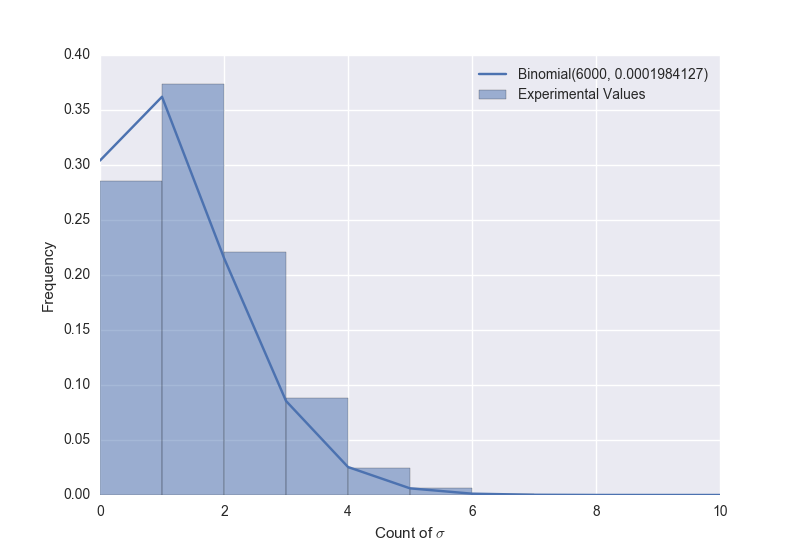
\includegraphics[scale=0.75]{./distx.png}
            \caption{Distribution of $X$}
            \label{fig:distx}
        \end{figure}

        In Figure~\ref{fig:distx} we can see that the theoretical distribution
        of $X$ matches the simulated values almost perfectly. This makes sense,
        and we would predict this to be the case. It's interesting that the
        simulated number of zero elements is lower than our distribution
        predicts, but that just goes to show the issues with simulated
        distributions.

        @ Use your algorithm to obtain $k$ independent realizations of $Y$ and
        obtain the histogram associated with these. How does the resulting
        histogram compare to the theoretical histogram of $Y$. Explain. Display
        the histogram and the theoretical distribution on the same plot. Make
        sure to comment on any expected or unexpected behavior.

        \begin{figure}[H]
            \centering
            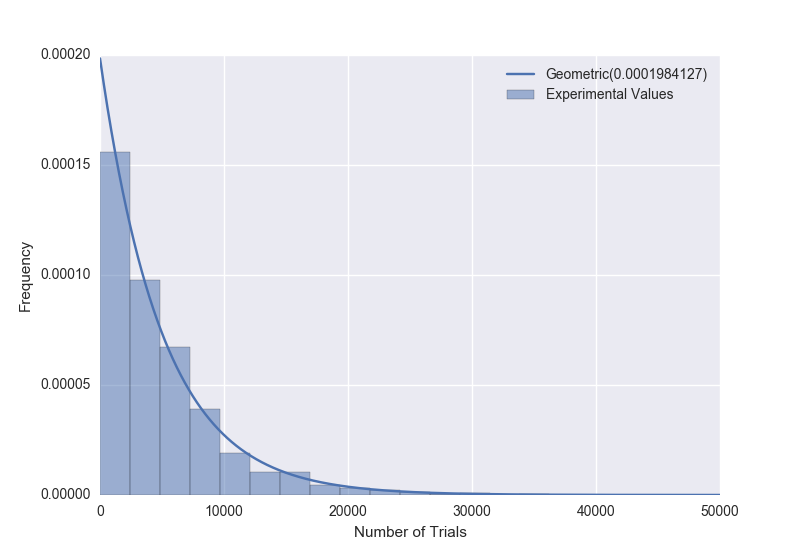
\includegraphics[scale=0.75]{./disty.png}
            \caption{Distribution of $Y$}
            \label{fig:disty}
        \end{figure}

        In Figure~\ref{fig:disty} we see that (as before with the distribution
        of $X$) the theoretical distribution of $Y$ matches our theory almost
        perfectly. There are some slight imperfections in the simulated values
        that lead to some mis-matched values, however on the whole these values
        are very close.
    \end{easylist}

\section{Part 2: Comparing Performance of Retrieving Algorithms}
Imagine you have an oracle that always answers the truth to a YES/NO question.
Suppose also you have a database with $n$ entries and that your goal is to
retrieve a special entry by asking questions to the oracle. Assume the database
is a permutation of the elements $\cren{1, \ldots, n}$ and that you want to
retrieve the position where the element $1$ is located.

Here are two methods:

\begin{easylist}[itemize]
    @ Iterate and ask about each item
    @ Binary tree and ask about each half.
\end{easylist}

Let $Q_A$ denote the total number of questions made to the oracle to determine
the position of $1$ using method A. Define $Q_B$ similarly. 

\subsection{Questions}

\begin{easylist}[enumerate]
    @ Determine $\mathbb{E}\pren{Q_A}$ explicitly. Justify with mathybits.

    \vspace{0.25cm}
    $\mathbb{E}\pren{Q_A} = (n / 2) + 1$. This can be seen by the following.
    Assume that for any given random permutation of our set $\mathcal{S}$, the
    value that we're looking for could be at any position, with uniform
    distribution.  Therefore, the average position is at the halfway mark. This
    means that on average, if an infinite number of trials occur with our value
    placed at a uniformly distributed random location location for each trial,
    the average point will be $(n / 2) + 1$. Note, it's not simply $n / 2$, as
    we always have to ask at least one question.

    @ Fix $n = 9$ and use your algorithm in the first part to simulate
    ten-thousand times the random variable $Q_A$. Determine the sample average
    of your simulations. Repeat with $n=21$, $n=36$, and $n=69$.

    \weave
    \inputminted[firstline=20,lastline=24]{python}{lab1_part2.py}
    \noweave

    @ How do the averages compare to your answer in part 1? Summarize your data in
    a table.  Comment on any expected and/or expected behavior.

    \begin{table}[H]
        \centering
        \begin{tabular}{|c|c|c|}
            \hline
            $n$ & $\mathbb{E}(Q_A)$ & Average Iterations\\
            \hline
            9  & $4.5$  & 5.00357\\
            21 & $10.5$ & 10.98759\\
            36 & $18$   & 18.48431\\
            69 & $34.5$ & 34.93481\\
            \hline
        \end{tabular}
        \caption{Method A Simulated Runtime}
        \label{table:methoda}
    \end{table}

    We see that this is almost exactly what we predicted. Interestingly, our
    values are higher than we'd expect, but this may be a result of the
    simulation process and errors that occur as a result.

    @ What should $\mathbb{E}\pren{Q_B}$ be approximately when $n$ is large?

    \vspace{0.25cm}
    $\mathbb{E}\pren{Q_b} = \log_2(n)$. This can be intuitively inferred from
    realizing that we are constructing a binary tree with depth $\log_2(n)$ when
    we examine the question space.

    @ Repeat 2 above but with $Q_B$ instead of $Q_A$.

    \weave
    \inputminted[firstline=27,lastline=49]{python}{lab1_part2.py}
    \noweave

    @ How do the obtained averages compare to your approximation in part 4?
    Summarize in a table and comment.

    \begin{table}[H]
        \centering
        \begin{tabular}{|c|c|c|}
            \hline
            $n$ & $\mathbb{E}(Q_B)$ & Average Iterations\\
            \hline
            9  & $3.1699$ & 3.22071\\
            21 & $4.3923$ & 4.47676\\
            36 & $5.1699$ & 5.22242\\
            69 & $6.1085$ & 6.14644\\
            \hline
        \end{tabular}
        \caption{Method A Simulated Runtime}
        \label{table:methoda}
    \end{table}

    We see that theory here matches our simulated values. This is good. This is
    exactly as we expected. As the description points out, this is because of
    the binary tree theory.

\end{easylist}

\newpage
\appendix
\section{Code}\label{app:code}

\subsection{Part 1}
\inputminted{python}{lab1_part1.py}

\subsection{Part 2}
\inputminted{python}{lab1_part2.py}

\end{document}
